\chapter{Minh họa kết quả suy luận của cử chỉ}
\label{Appendix3}

\section{So sánh giữa cử chỉ ground truth và cử chỉ dự đoán}


\begin{center}
\centering
\href{https://youtu.be/22lNm2tvmrk}{% Replace with your YouTube URL
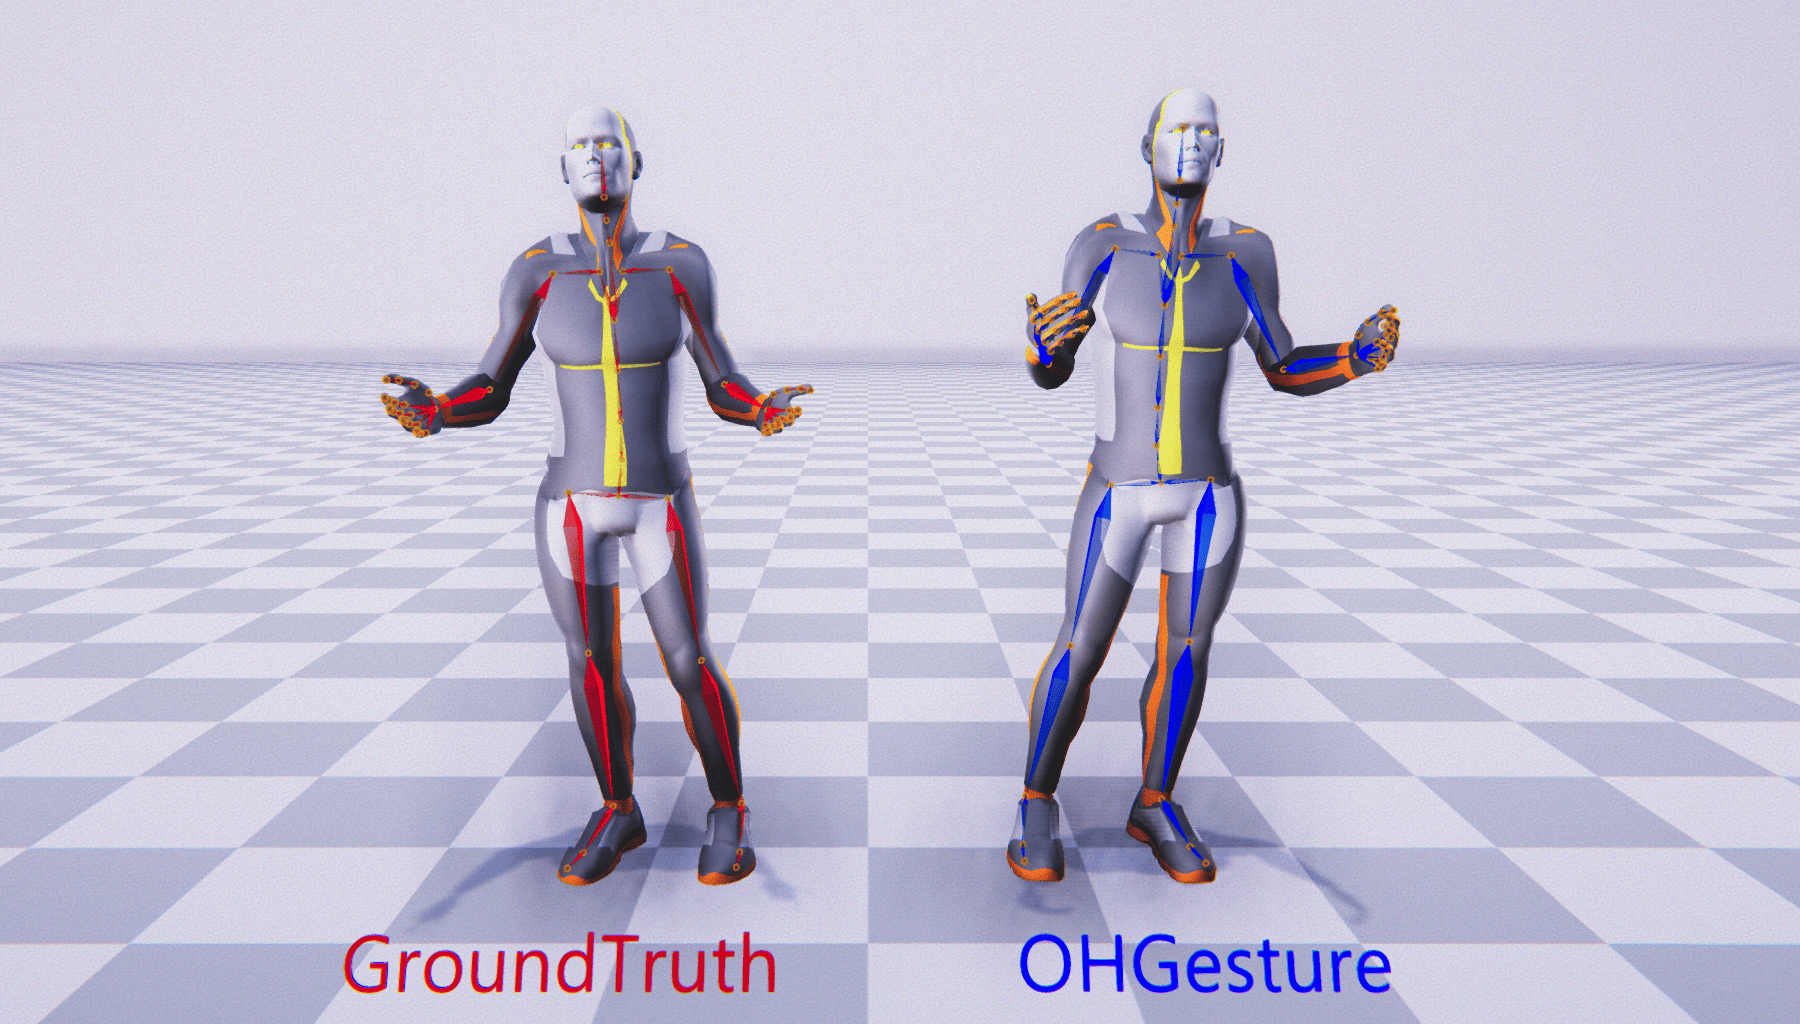
\includegraphics[width=\textwidth]{GroundTruthCompare}}
{\tiny Click vào ảnh để xem video}
\end{center}

Kết quả cử chỉ ground truth và cử chỉ dự đoán của mô hình ở frame $3821$ dự đoán trên mẫu giọng nói $\texttt{003\_Neutral\_2\_x\_1\_0}$

\section{Minh họa các cảm xúc khác nhau của cử chỉ}

{
	\begin{center}
		\centering
		\href{https://youtu.be/KUlBZXLtYJ4}{% Replace with your YouTube URL
			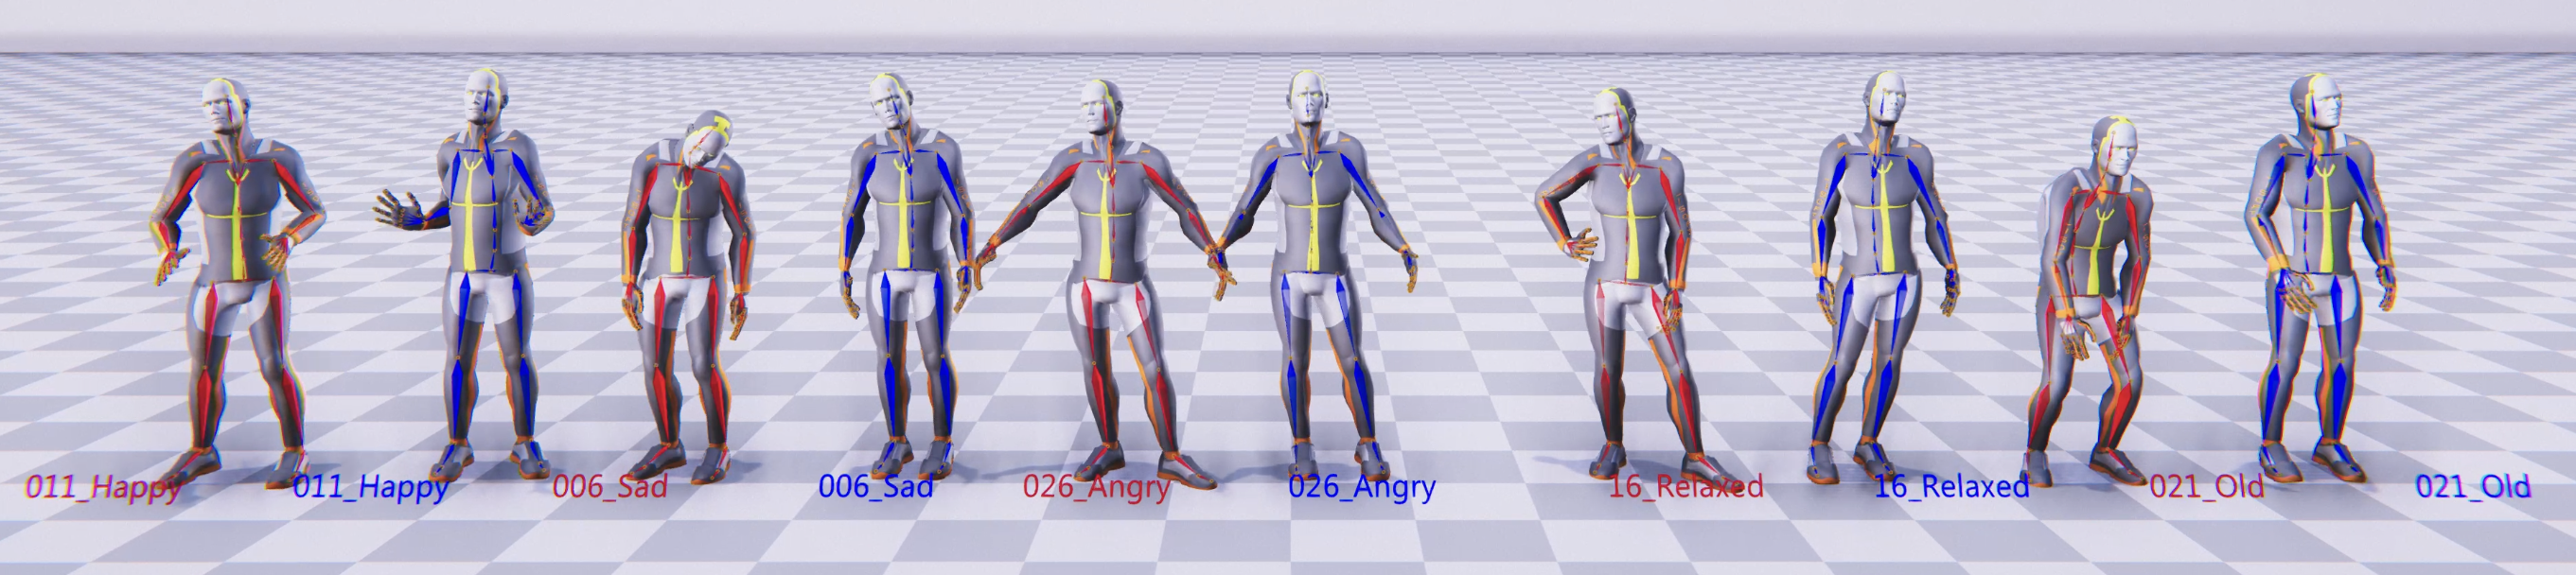
\includegraphics[width=\textwidth]{DifferenceEmotion}}
		
		{\tiny Click vào ảnh để xem video}
	\end{center}
}

Kết quả sinh hay suy luận của mô hình OHGesture với các cảm xúc khác nhau. Màu đỏ là ground truth trong tập dữ liệu ZeroEGGS, màu xanh là kết quả sinh của mô hình OHGesture.

{
	\begin{center}
		\centering
		\href{https://youtu.be/eZghfNGmZn8}{% Replace with your YouTube URL
			\includegraphics[width=\textwidth]{ListOfEmotion}}
		
		{\tiny Click vào ảnh để xem video}
	\end{center}
}

\section{Minh họa việc sinh cử chỉ với giọng nói nằm ngoài tập huấn luyện}

{
	\begin{center}
		\centering
		\href{https://www.youtube.com/watch?v=B6nv1kQmi-Q}{% Replace with your YouTube URL
		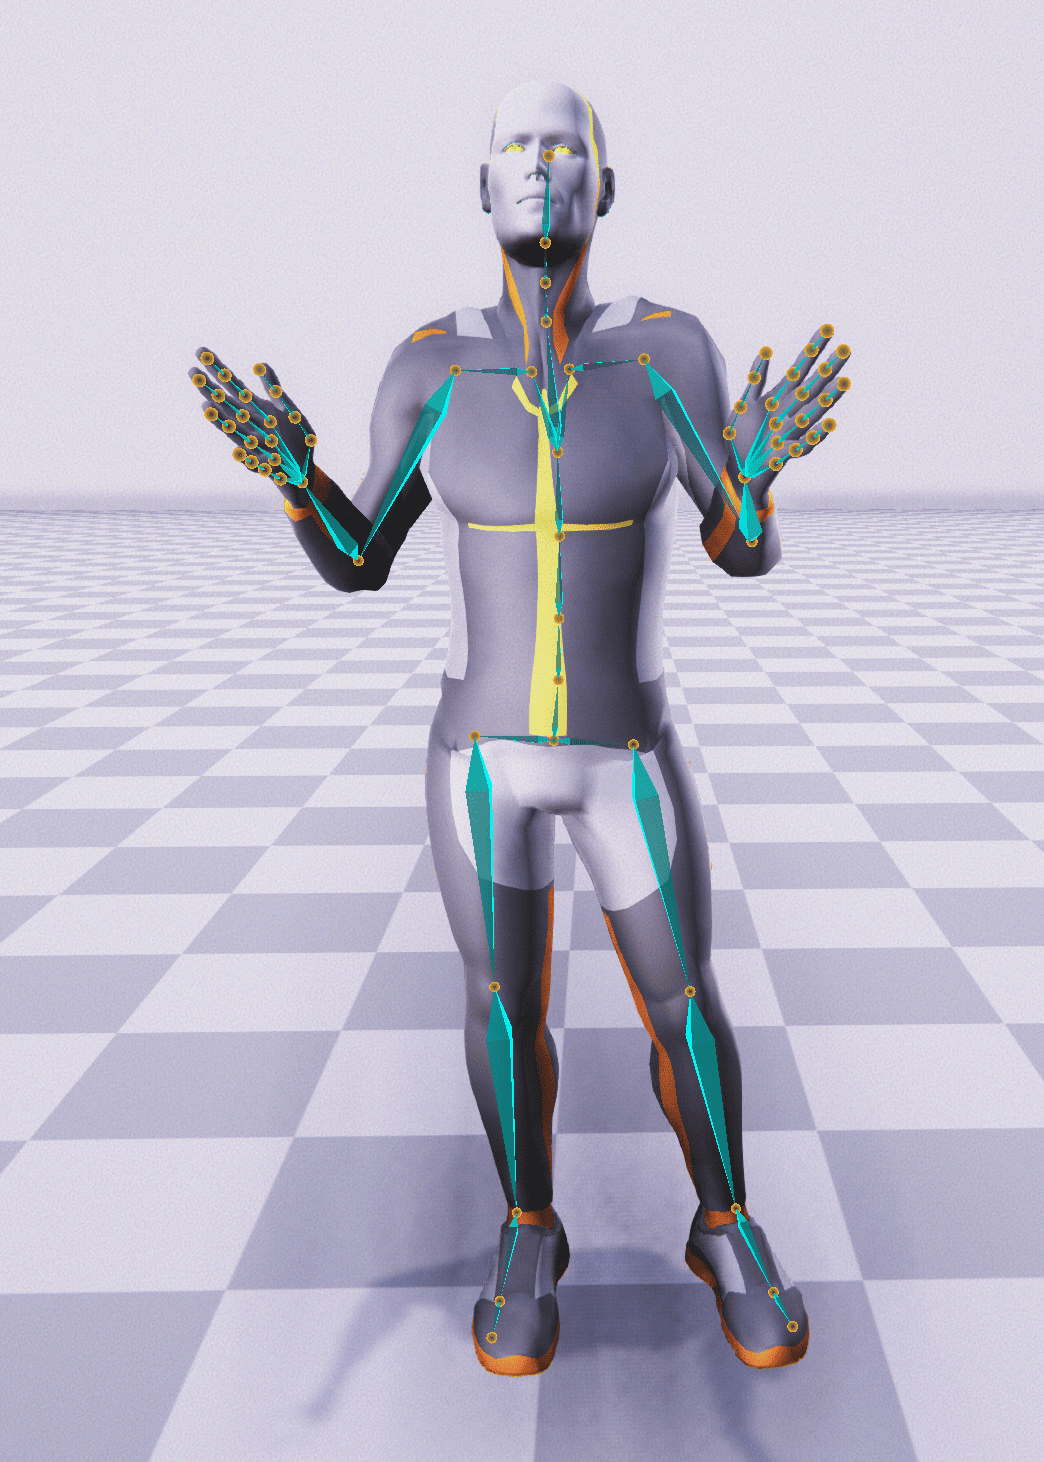
\includegraphics[width=0.4\textwidth]{StevenJob}}
		
		{\tiny Click vào ảnh để xem video}
	\end{center}
}

Minh họa sinh cử chỉ tương ứng với giọng nói của Steve Job


{
	\begin{center}
		\centering
		\href{https://youtu.be/yLwXdm7UgPE}{% Replace with your YouTube URL
			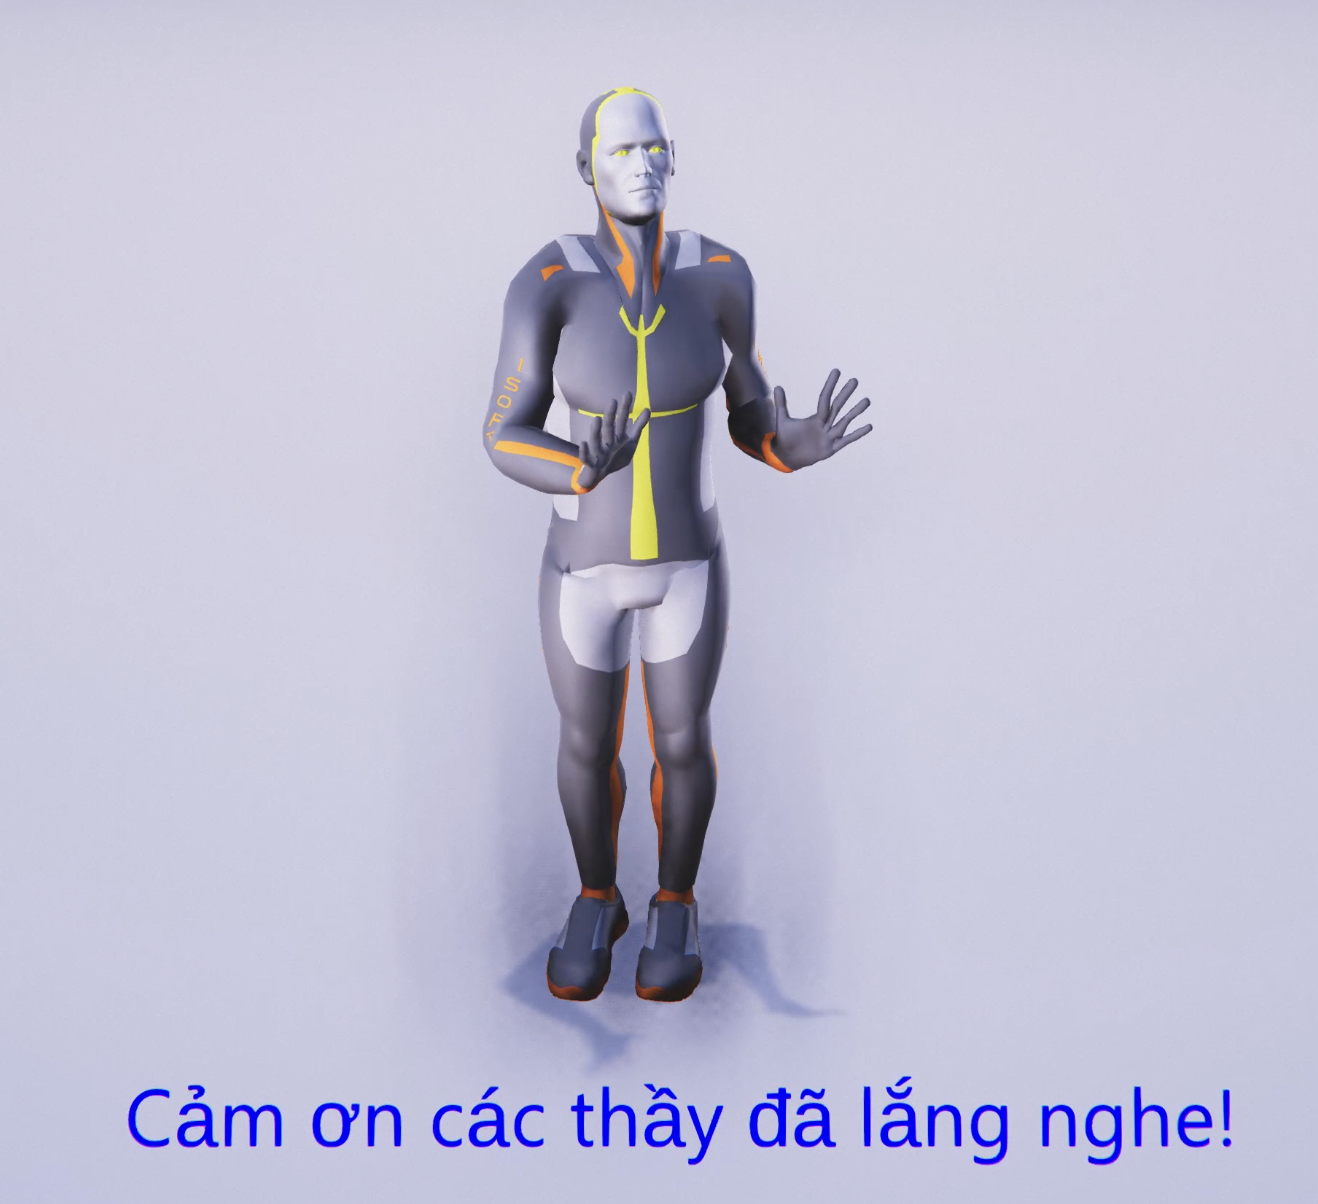
\includegraphics[width=0.6\textwidth]{OHGestureDemo}}
		
		{\tiny Click vào ảnh để xem video}
	\end{center}
}

Minh họa sinh cử chỉ với giọng nói được tạo từ Microsoft Azure giới thiệu về đề tài.

\section{Minh họa chuyển động của nhân vật}

\begin{center}
{
	\centering
	\href{https://www.youtube.com/watch?v=9IIIZP3EJLg}{% Replace with your YouTube URL
	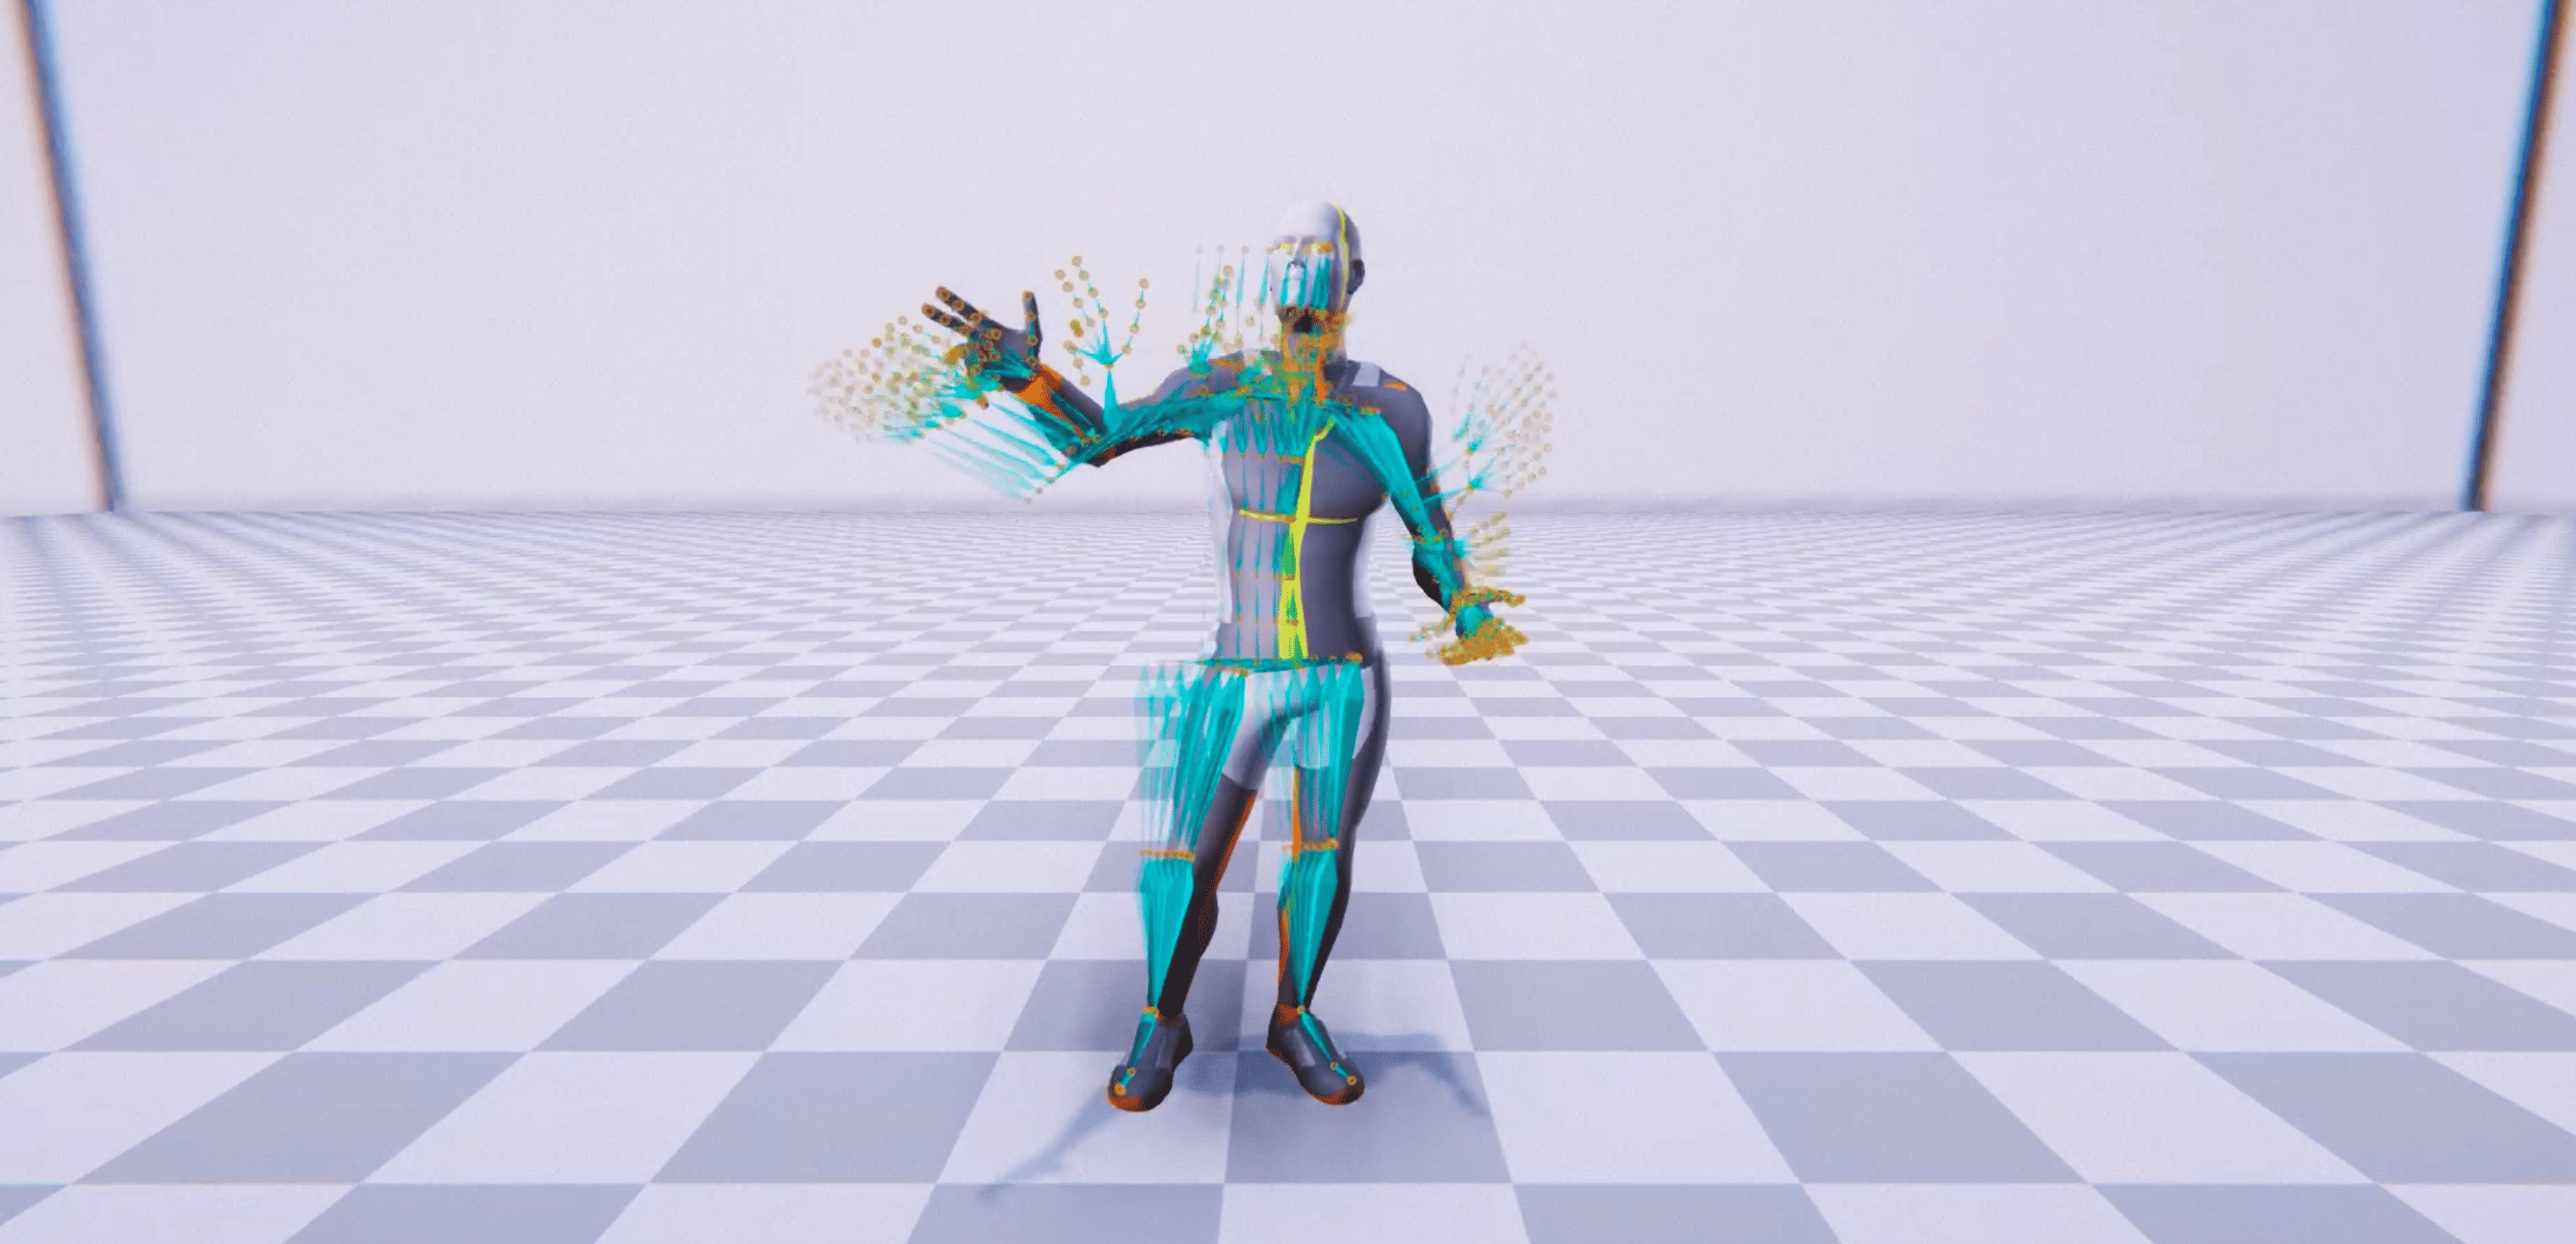
\includegraphics[width=0.8\textwidth]{DemoMotionGesture}}
	
	{\tiny Click vào ảnh để xem video}
}
\end{center}
Minh họa cử chỉ được lấy 6 khung hình phía trước và 6 khung hình phía sau của cử chỉ.